\subsection{动态规划求解01背包问题}
\subsubsection{算法类别}
此处介绍的01背包问题解法是一种动态规划方法.

\subsubsection{算法思路}
\paragraph{0-1背包问题的子问题描述}

设所给01背包问题的子问题为
\begin{equation}
	\max \sum^n_{k=i}{v_k x_k}
	\label{eq:01bp}
\end{equation}

其限制条件为

\begin{equation}
	\left\{
	\begin{array}{rl}
		\sum^n_{k=i}{w_kx_k\leq j} \\
		x_k\in \{0,1\}, i\leq k\leq n
	\end{array}
	\right.
	\label{eq:01bp-limit}
\end{equation}

\paragraph{0-1背包问题的最优子结构性质}
容易证明0-1背包问题具有最优子结构性质:
设0-1背包问题的子问题\ref{eq:01bp}的最优值为$m(i, j)$, 即$m(i, j)$是背包容量为j,
可选择物品为$i, i+1, \dots, n$的时候的最优值.\par

设$(y_1, y_2, \dots, y_n)$是$x_i \tilde x_n$的一个最优解, 则可以推断, $(y_2,
	y_3, \dots, y_n)$是一个子问题\ref{eq:01bp-sub-problem}的最优解.\par

\begin{equation}
	\max \sum^n_{i=2}{v_i y_y}
	\label{eq:01bp-sub-problem-1}
\end{equation}

\begin{equation}
	\left \{
	\begin{array}{rl}
		\sum^n_{i=1}w_i y_i \leq C-w_1y_1 \\
		y_i \in \{0,1\}, 1\leq i \leq n
	\end{array}
	\right.
	\label{eq:01bp-sub-problem}
\end{equation}

否则, 假设$(y_2, y_3, \dots, y_n)$不是子问题的最优解, 则存在一组$(y_2',
	y_3', \dots, y_n')$是子问题式\ref{eq:01bp-sub-problem}的最优解, 则$(y_1, y_2',
	y_3', \dots, y_n')$是原问题的最优解, 矛盾. 因此$(y_2, y_3, \dots,
	y_n)$是原问题的最优解. 0-1背包问题的最优子结构得证.

据此, 可得0-1背包问题的计算$m(i, j)$的递归式(状态转移方程)如下:
\begin{equation}
	m(i,j)=\left\{
	\begin{array}{rl}
		max\{m(i+1,j), m(i+1,j-w_i)+v_i\}, & j\geq w_i     \\
		m(i+1,j)                         , & 0\leq j < w_i
	\end{array}
	\right.
\end{equation}

\begin{equation}
	m(n,j)=\left\{
	\begin{array}{rl}
		v_n, & j\geq w_n     \\
		0  , & 0\leq j < w_n
	\end{array}
	\right.
\end{equation}


\subsubsection{关键函数及代码段的描述}
采用动态规划的方式实现0-1背包问题.\par

其核心代码实现如下:

\begin{lstlisting}[language=c++]
void BackPack01::backPackDP() {
    maxVal = -1;

    // Initialize
    for (int j = 0; j <= volume; j++) {
        dp[n - 1][j] = (j >= w[n - 1]) ? val[n - 1] : 0;
    }

    int i = n - 2, j = volume;
    for (; i >= 0; i--) {
        j = volume;
        for (; j >= 0; j--) {

            // Compare total value of items in the backpack between put
            // item[i] in and not put it in.
            dp[i][j] = (j >= w[i]) ? std::max(dp[i + 1][j],
                                              dp[i + 1][j - w[i]] + val[i])
                                   : dp[i + 1][j];
        }
    }

    maxVal = dp[0][volume];
}
\end{lstlisting}

\subsubsection{算法时间及空间复杂性分析}
\paragraph{空间复杂度分析}
0-1背包问题的动态规划实现需要一个大小为N*C的数组进行辅助,
所以空间复杂度为$O(NC)$.

\paragraph{时间复杂度分析}
由于动态规划的本质是上述递推式\ref{eq:01bp-sub-problem},
且实现的核心代码使用了两层循环, 所以可以很方便的计算出时间复杂度为

\begin{equation}
	C(n) = O(N)\times O(C) = O(NC)
\end{equation}

% \begin{gather}
% 	C'(0) = 0            \nonumber \\
% 	C'(k) = 2C'(k-1)+2^k \nonumber
% \end{gather}
综上, 0-1背包问题的一般动态规划解法的时间复杂度为O(NC).

\subsection{应用跳跃点方法优化的0-1背包问题动态规划解法}
\subsubsection{算法类别}
应用了跳跃点方法优化的0-1背包问题解法也是一种动态规划方法.

\subsubsection{算法思路}
\label{sec:jumpPointThink}
\paragraph{概述}
由$m(i, j)$的递归式容易证明, 在一般的情况下, 对每一个确定的$i(1\leq i\leq n)$,
函数$m(i, j)$是关于变量j的阶梯状单调不减函数. 跳跃点是这一类函数的描述特征.
在一般情况下, 函数$m(i, j)$由其全部跳跃点唯一确定. 如图所示.

\begin{figure}[ht!]
	\centering
	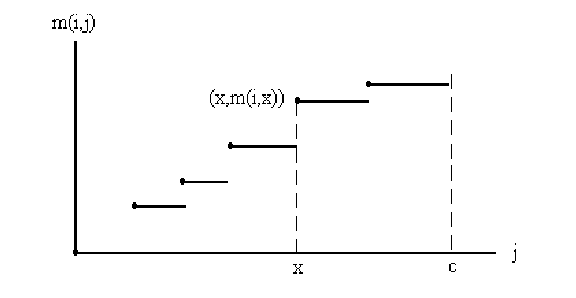
\includegraphics[width=0.8\textwidth]{figures/JumpPoint.png}
	\caption{跳跃点}
	\label{fig:JumpPoint}
\end{figure}

对每一个确定的$i,(1\leq i\leq n)$, 用一个链表p[i]存储函数$m(i,j)$的全部跳跃点.
链表p[i]可以计算$m(i,j)$的递归式递归地由表p[i+1]计算,
初始的时候p[n+1]=\{(0,0)\}.

\paragraph{算法改进的描述}
函数$m(i,j)$是由函数$m(i+1,j)$与函数$m(i+1, j-w_i)+v_i$作max运算得到的. 因此,
函数$m(i,j)$的全部跳跃点包含于函数$m(i+1,j)$的跳跃点集p[i+1]与函数
$m(i+1,j-w_i)+v_i$的跳跃点集q[i+1]的并集中.\par

易知, $(s,t)\in q[i+1]$当且仅当$w_i\leq s\leq c$且$(s-w_i,t-v{i})\in p[i+1]$. \par

因此, 容易由p[i+1]确定跳跃点集q[i+1]如下:
\begin{equation}
	q[i+1]=p[i+1]\oplus (w_i,v_i)=\{(j+w_i,m(i,j)+v_i)|(j,m(i,j))\in p[i+1]\}
	\label{eq:jumpSet}
\end{equation}

另一方面, 设(a,b)和(c,d)是$p[i+1]\cup q[i+1]$中的2个跳跃点, 则当$c\geq
	a$且$d<b$的时候, (c,d)受控于(a, b), 从而(c, d)不是p[i]中的跳跃点.
除了受控跳跃点之外, $p[i+1]\cup q[i+1]$中的其他跳跃点都是p[i]中的跳跃点.\par

由此可见, 在递归地由表p[i+1]计算表p[i]的时候, 可以先由p[i+1]计算出q[i+1],
然后合并表p[i+1]和表q[i+1], 并清除其中的受控跳跃点得到表p[i].

\subsubsection{关键函数及代码段的描述}
使用跳跃点优化的动态规划方法求解0-1背包问题的关键在于根据上述推导过程动态
根据上一状态的跳跃点集维护当前状态的跳跃点. 具体代码如下:\par
对函数均使用类似C++的Pseudo-Code描述.

\begin{lstlisting}[language=c++]
void BackPackJumpPoint::JumpPointBackPackDP() {
    int *head = new int[n + 2]; // Track jump point start position.
    head[n] = 0;
    jp[0][0] = 0; // Store item weight
    jp[0][1] = 0; // Store item value

    // Left points to first jump point of p[i+1], right points to last jump
    // point of p[i+1]. Next is position where next jump point will store.
    int left = 0, right = 0, next = 1;
    head[n - 1] = 1; // Points to the position of first jump point of item[n-1].

    for (int i = n - 1; i >= 0; i--) {
        int k = left; // k points to jump points of p[], move k to
                      // evaluate controlled points in p[] and
                      // p[]+(w,v)
        for (int j = left; j <= right; j++) {

            if (jp[j][0] + w[i] > volume) {
                // No enough backpack space to fit item[i] in, exit loop.
                break;
            }

            // Compute new jump point as jp[]+(w,v).
            int x = jp[j][0] + w[i];
            int y = jp[j][1] + val[i];

            // If jp[k][0] < x, then it must be a jump point of current
            // item.
            while (k <= right && jp[k][0] < x) {
                jp[next][0] = jp[k][0];
                jp[next++][1] = jp[k++][1];
            }

            // Clear controlled jump point.
            if (k <= right && jp[k][0] == x) {
                if (y < jp[k][1]) {
                    y = jp[k][1];
                }
                k++;
            }

            if (y > jp[next - 1][1]) {
                jp[next][0] = x;
                jp[next++][1] = y;
            }

            while (k <= right && jp[k][1] <= jp[next - 1][1]) {
                k++;
            }
        }

        // Add remaining jump points.
        while (k <= right) {
            jp[next][0] = jp[k][0];
            jp[next++][1] = jp[k++][1];
        }

        left = right + 1;
        right = next - 1;

        head[i - 1] = next;
    }


    maxVal = jp[next - 1][1];
}
\end{lstlisting}

\subsubsection{算法时间及空间复杂性分析}
\paragraph{空间复杂度分析}
\label{par:jumpPointSpace}
相比于一般的动态规划解0-1背包算法,
应用跳跃点法的动态规划解0-1背包算法额外使用数组存储了跳跃点,
这一部分是空间的主要支出, 从跳跃点集p[i]的定义可以看出,
p[i]中的跳跃点相应于$x_i, \dots, x_n$的0/1赋值, 因此,
p[i]中的跳跃点个数不超过$2^{n-i+1}$. 又由于受控跳跃点会被清除, 因此,
跳跃点集最多使用$O(min\{N\times 2^{N}, c\})$的额外空间.\par

由于跳跃点表p[i]的计算只依赖于p[i+1]的数据,
所以p[i+2]及之后的跳跃点表不需要保存,
这样就将跳跃点表的大小从$O(min\{N\times 2^N, c\})$优化到了$O(min\{2^N, c\})$.

\paragraph{时间复杂度分析}
\label{par:jumpPointTime}
跳跃点算法的主要计算量在于计算跳跃点集$p[i](1\leq i\leq n)$.
由于$q[i+1]=p[i+1]\oplus (w_i,v_i)$, 故计算q[i+1]需要$O(|p[i+1]|)$的计算时间.
合并p[i+1]和q[i+1]并清除受控跳跃点也需要$q[i+1]=p[i+1]\oplus
	(w_i,v_i)$的计算时间. 从跳跃点集p[i]的定义可以看出,
p[i]中的跳跃点相应于$x_i,\dots,x_n$的0/1赋值. 因此,
p[i]中的跳跃点个数不超过$2^{n-i+1}$. 由此可见,
算法计算跳跃点集p[i]所花费的计算时间为

\begin{equation}
	O(\sum^n_{i=2}|p[i+1]|)=O(\sum^n_{i=2}2^{n-i})=O(2^n)
	\label{eq:jumpPointTime}
\end{equation}

从而, 改进后算法的计算时间复杂性为$O(2^n)$. 当所给物品的重量$w_i(1\leq i\leq n)$
是整数的时候, $|p[i]|\leq c+1, (1\leq i\leq n)$. 在这种情况下,
改进后的算法的计算时间复杂度为$O(min\{nc, 2^n\})$.

% \begin{align}
% 	C(1)       & = 0                        \nonumber \\
% 	C_{min}(n) & = 2C(\frac{n}{2}) + n - 1  \nonumber \\
% 	C_{max}(n) & = C(1) + C(n - 1) + n - 1  \nonumber
% \end{align}
